\documentclass{beamer}
\usetheme{Boadilla}
\usepackage{mathtools}
\usepackage{amssymb}
\usepackage{amsfonts}
\usepackage{amsmath}
\usepackage{breqn}
\usepackage{wrapfig}
\usepackage{floatflt}

\title{EC607 Public Presentation}
\author{Melissa Wilson}
\institute{University of Oregon}
\date{\today}

\begin{document}

\begin{frame}
\titlepage
\end{frame}

\begin{frame}
\frametitle{}
{\bf ``The Impact of Family Income on Child Achievement: Evidence from the Earned Income Tax Credit''} \\
Gordan B. Dahl and Lance Lochner (American Economic Review, 2012)
\end{frame}


\section{Introduction}


\begin{frame}
\frametitle{Introduction I}
\begin{itemize}
	\item This paper analyzes the effects of income on children's math and reading achievement by exploiting large, nonlinear changes in the Earned Income Tax Credit (EITC) using a panel of 4,412 children matched to their mothers
	\item Expansions of the EITC in the late 1980s and 1990s provide an exogenous source of variation in income, so the authors use this to overcome the problems caused by the endogeneity of income and identify true causal effects
	\item Use a first-differenced child outcome equation and implement IV approach outlined later
	\item Affirms importance of family income effects on child academic achievement and shows it is heterogeneous across family income levels
\end{itemize}
\end{frame}


\section{Background}


\begin{frame}
\frametitle{Background}
\begin{itemize}
	\item Prior literature shows significant variation in estimated effects of family income on child development
	\item Estimates are mostly positive and significant, but magnitude changes
	\item The direction of the relationship may be clear, but the causal relationship has not been identified due to omitted variable bias due to heterogeneous unobservable home-life characteristics 
	\item Some have used FE in order to overcome this, but they do not control for endogenous transitory shocks
	\begin{itemize}
		\item Eg. job loss, promotion, family illness, moving, etc.
		\item Likely suffer from attenuation bias because income growth is measured noisily
	\end{itemize} 
\end{itemize}
\end{frame}


\section{Methodology}


\begin{frame}
\frametitle{Methodology I}
\begin{itemize}
	\item Child outcome equation:
	\begin{equation}
		y_{ia} = x_i^' \alpha_a + w_{ia}^' \beta + I_{ia}\delta_0 + I_{i, a-1}\delta_1 + \dots + I_{i, a-L}\delta_L + \mu_i + \epsilon_{ia} 
	\end{equation}
	for child $i$ at age $a$ with $L$ lags %w are time-varying characteristics and I is net family income
	\item Taking first differences and setting $L=0$ gives the baseline equation:
	\begin{equation}
		\Delta y_{ia} = x_i^' \alpha + \Delta w_{ia}^' \beta + \Delta I_{ia}\delta_0 + \Delta \epsilon_{ia}
	\end{equation}
	where $ \alpha \equiv \alpha_a - \alpha_{a-1} $ is the effect of $x_i$ on achievement growth
	\item Assuming $L=0$ gives the ``contemporaneous effects" of family income on children, ignoring long-run effects
	\item Authors will allow one- and two-year lags, as well after baseline model
\end{itemize}
\end{frame}

\begin{frame}
\frametitle{Methodology II}
\begin{itemize}
	\item Primary concern with OLS is that $\Delta \epsilon_{ia}$ may be correlated with entire history of family income
	\item Employ instrumental the following variable approach
	\item EITC income is a function of pretax income and taxes:
	\begin{equation*}
		I_{ia} = P_{ia} + \chi_a^{s_{ia}}(P_{ia}) - \tau_a^{s_{ia}}(P_{ia})
	\end{equation*}
	\item Use IV:  
	\begin{equation*}
		\Delta \chi_a^{IV}(P_{i, a-1}) \equiv \chi_a^{s_{i, a-1}}(\hat{E}\left[P_{i,a} | P_{i, a-1} \right]) -  \chi_a^{s_{i, a-1}}(P_{i,a-1})
	\end{equation*}
	where $ \hat{E}\left[P_{i,a} | P_{i, a-1} \right] $ is an estimate of pretax income given lagged pretax income
	\item Also use flexible function of lagged pretax income when instrumenting
	\item This builds on IV used in Gruber and Saez (2002)
\end{itemize}
\end{frame}

\begin{frame}{Methodology III}
	Thus, IV estimation is of the following equation
	\begin{equation}
		\Delta y_{ia} = x_i^' \alpha + \Delta w_{ia}^' \beta + \Delta I_{ia} \delta_0 + \Phi(P_{i, a-1}) + \eta_{ia}
	\end{equation}
\end{frame}

\begin{frame}{Methodology IV}
	\begin{itemize}
		\item Assumes the relationship between child development shocks and lagged pretax income must be stable over time
		\item Identification from differential changes in EITC schedule over time
		\item Minor issues with data and model:
		\begin{enumerate}[(1)]
			\item Vast majority of EITC recipients receive their credit after filing taxes the following year; thus, authors link test scores with income earned in previous year
			\item Only observe child achievement scores every other year; thus, authors year two-year differences
		\end{enumerate}
	\end{itemize}
\end{frame}

\section{Data}


\begin{frame}
\frametitle{Data I}
\begin{itemize}
	\item Use data from National Longitudinal Survey of Youth (NLSY)
	\item Links children to their mothers and follows families over time, allowing use of child FEs
	\item Repeated measures of academic achievement and family income
	\item Oversamples minority families, providing a larger sample of families eligible for EITC
	\item Note that the NLSY does not provide information on how much a family receives from EITC, so authors must approximate this based on IRS (2002) and Scholz (1994) estimates that 80-87\% of eligible HH receive EITC
	\item Authors assume full take-up and impute each family's state and federal EITC payment and tax burden using the TAXSIM program from the NBER
\end{itemize}
\end{frame}

\begin{frame}
\frametitle{Data II}
\begin{itemize}
	\item Restrict sample to children observed in at least two consecutive survey years, since using FEs
	\item Restrict sample to those children whose mothers did not change marital status between test score measures
	\item Noticeable income increase in sample (increases faster than price levels) and show it is largely attributable to mothers in the sample aging
	\item Average child age in sample is 11
	\item Over half of sample are minorites due to oversampling of minorities in NSLY
\end{itemize}
\end{frame}


\section{Results}


\begin{frame}
\frametitle{OLS Results I}
	\begin{figure}
		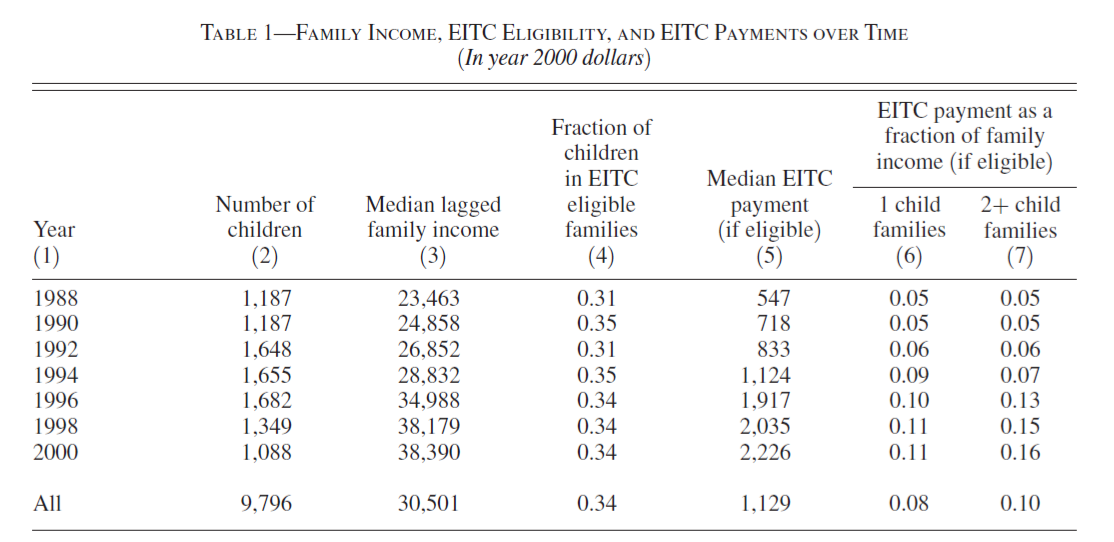
\includegraphics[scale=0.3]{..\Tables\table1.png} %unit of change in income is $1000
	\end{figure}
\end{frame}

\begin{frame}
\frametitle{OLS Results II}
	\begin{itemize}
		\item Possible reasons for discrepancy when including lags:
		\begin{enumerate}[(1)]
			\item Measurement error is greater for those measured in differences, so attenuation bias is greater for differenced estimates
			\item Correlation between unobserved FEs ($\mu_i$) and family income biasing cross-sectional OLS estimates 
		\end{enumerate}
		\item Both suffer from OVB due to transitory shocks
	\end{itemize}
\end{frame}

\begin{frame}
\frametitle{IV Estmates: Contemporaneous Effects}
	\begin{figure}
		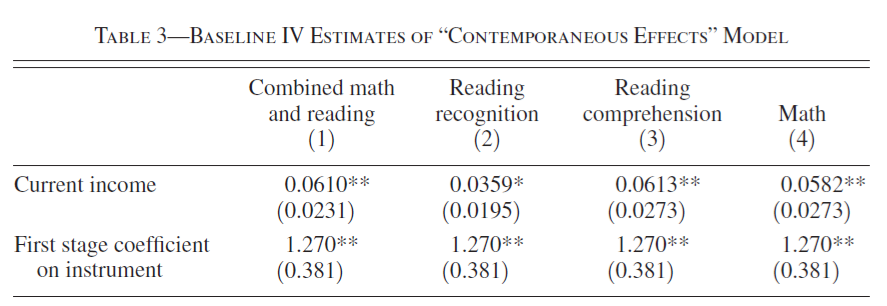
\includegraphics[scale=0.4]{..\Tables\table2.png}
	\end{figure}
\end{frame}

\begin{frame}
\frametitle{IV Results: Contemporaneous Effects}
\begin{itemize}
	\item Table 3 shows raising income by \$1000 increases math-reading achievement by 6 percent of a standard deviation (not very big, but larger than OLS)
	\item Table 4 takes into account national time trends and changes in state-level school accountability and welfare policies
	\item Authors use 
	\begin{enumerate}[A.]
		\item year dummies to allow for average test scores to vary year to year, so identification of IV estimate comes from differences in predicted EITC across individuals
		\item linear time trends
		\item linear time trend and interaction of trend with control function $\Phi()$ to account for relationship between child outcomes and pretax income changing over time
		\item  and 
		\item Address changes in state policies
	\end{enumerate} 
\end{itemize}
\end{frame}

\begin{frame}
\frametitle{IV Estimates: Contemporaneous Effects and Controls}
\begin{figure}
	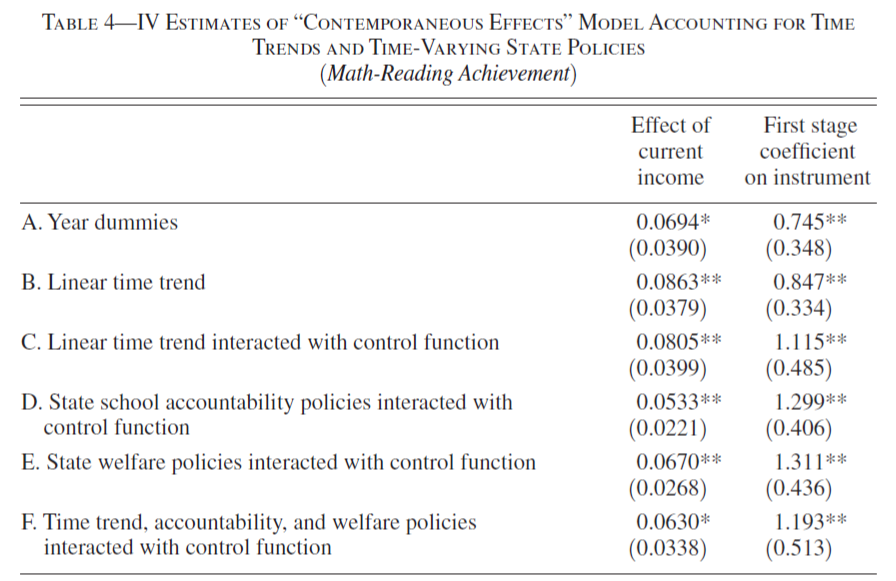
\includegraphics[scale=0.3]{..\Tables\table3.png} %Table 4
\end{figure}
\end{frame}

\begin{frame}
\frametitle{IV Estimates: Contemporaneous and Lasting Effects}
\begin{figure}
	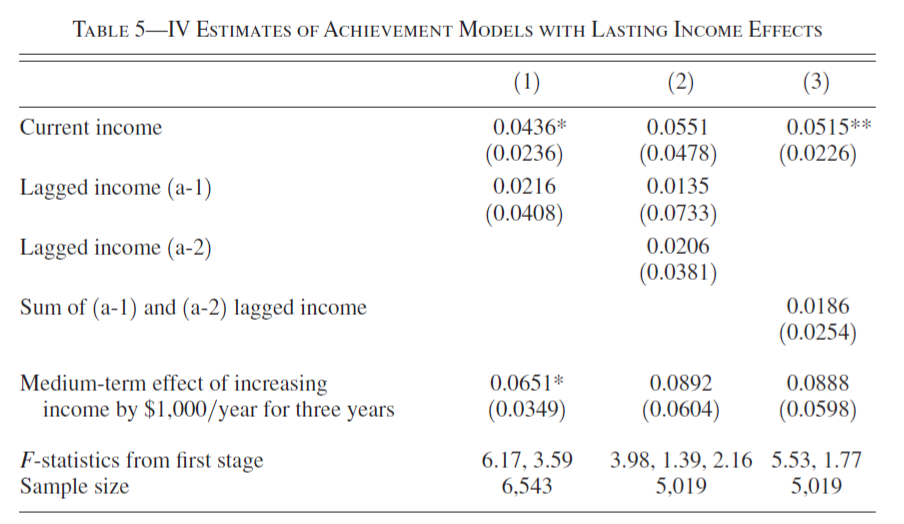
\includegraphics[scale=0.3]{..\Tables\table4.png} %Table 5
\end{figure}
\end{frame}

\begin{frame}
\frametitle{IV Results: Contemporaneous and Lasting Effects}
\begin{itemize}
	\item In table 5, the authors allow for lasting effects of income changes
	\item The results are largely consistent, but more precise
	\item Larger contemporaneous effects than lasting effects
	\item The simple "contemporaneous effects" model provides reasonable good estimates of short-run effects of income
\end{itemize}
\end{frame}

\begin{frame}
\frametitle{IV Estimates: Heterogeneous Effects}
\begin{figure}
	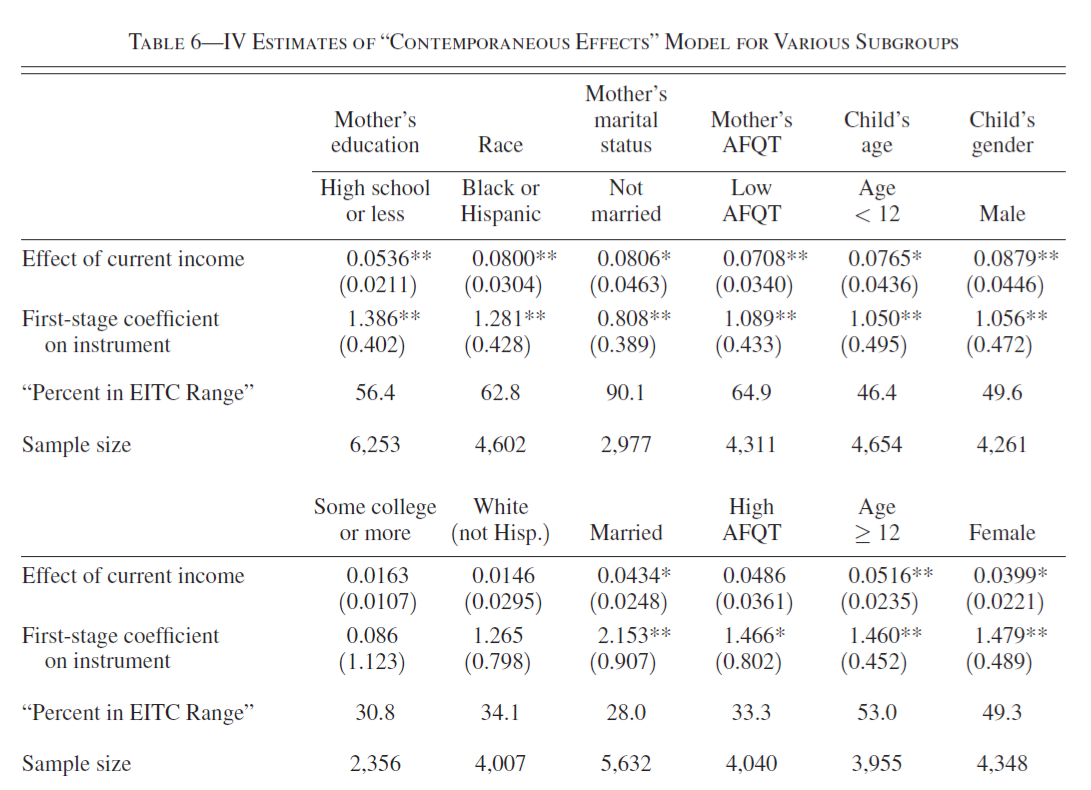
\includegraphics[scale=0.3]{..\Tables\table5.png} %Table 6
\end{figure}
\end{frame}

\begin{frame}
\frametitle{IV Results: Heterogeneous Effects}
\begin{itemize}
	\item The extent of the impact of a \$1000 increase in current income reported as ``Percent in EITC Range" for each subgroup
	\item Higher socioeconomic status (SES) groups have lower PEITCR
	\item This is reflected in higher SEs for those groups point estimates
\end{itemize}
\end{frame}


\section{Robustness}


\begin{frame}
\frametitle{Robustness I}
\begin{itemize}
	\item Include additional controls for parents and families
	\item Remove all controls from baseline
	\item Interact all baseline controls with pretax income and the polynomial lagged pretax income
	\item Show inclusion of state FEs has little impact
\end{itemize}
\end{frame}

\begin{frame}
\frametitle{Robustness II}
\begin{itemize}
	\item NLSY-created weights for initial sample of mothers to weight observations
	\begin{itemize}
		\item Smaller point estimate
		\item Larger SEs
	\end{itemize}
	\item Use log total family income as RHS, rather than levels
	\item Add changes to maternal LFP and hours worked to baseline
\end{itemize}
\end{frame}


\section{Conclusion}


\begin{frame}
\frametitle{Conclusion}
\begin{itemize}
	\item Exploiting exogenous variation in the EITC, the authors estimate that income has a modest positive contemporaneous effect on child academic achievement
	\item Baseline estimates imply that a \$1000 increase in family income raises math and reading comprehension scores by 6 percent of a standard deviation
	\item For the whole sample, this implies an average test score increase of 10 percent of a standard deviation based on EITC payments increasing income of two-child families by \$1670, on average
	\item Effects are larger for disadvantaged families, younger children, and boys 
\end{itemize}
\end{frame}



\iffalse
	\begin{columns}
		\column{0.5\textwidth}
		\centering
		%	\begin{figure}
		%		\includegraphics[scale=0.3]{fig5}
		%	\end{figure}
		\column{0.5\textwidth}
		\centering
		%	\begin{figure}
		%		\includegraphics[scale=0.3]{fig6}
		%	\end{figure}
	\end{columns}
\fi




\end{document}